\documentclass[12pt,twoside,book]{article}
\usepackage{docmute}

\input{../settings}

\begin{document}

%%%%%%%%%%%%%%%%%%%%%%%%%%%%%%%%%%%%%%%%%%%%%%%%%%%%%%%%%%%%%%%%%%%%%%%%%%%%%%%
\section{WIMP as a dark matter}
\setcounter{equation}{0}
%%%%%%%%%%%%%%%%%%%%%%%%%%%%%%%%%%%%%%%%%%%%%%%%%%%%%%%%%%%%%%%%%%%%%%%%%%%%%%%

\vskip 0.1in

%%%%%%%%%%%%%%%%%%%%%%%%%%%%%%%%%%%%%%%%%%%%%%%%%%%%%%%%%%%%%%%%%%%%%%%%%%%%%%%
\subsection{WIMP dark matter relic abundance}
%%%%%%%%%%%%%%%%%%%%%%%%%%%%%%%%%%%%%%%%%%%%%%%%%%%%%%%%%%%%%%%%%%%%%%%%%%%%%%%

One of the most important evidences of the beyond SM is the existence of
dark matter (DM) \cite{Zwicky:1933}.  DM is an unknown object that
occupies a non-negligible ratio of the total energy of our universe, but
has not yet been directly observed because of its weak interaction with
the SM particles.\footnote{
%%
At worst DM interacts with the SM particles through the gravity, which
is considerably weaker than all the other known interactions.
\rem{Mention to Ema paper??}
}
%%
In spite of its invisibility, the existence of DM is confirmed by
several astrophysical observations such as the mass measurement using
the gravitational lensing effect caused by galaxies and clusters
\cite{Zwicky:1937, Trimble:1987ee}, the flatness of galactic rotation
curves further the optical radius \cite{1939LicOB..19...41B,
Begeman:1991iy}, the measurement of the power spectrum of the cosmic
microwave background (CMB), and so on.  In particular, the observation
of CMB allows us the precise determination of various cosmological
parameters \cite{Jungman:1995av, Jungman:1995bz} including the density
of the non-relativistic matter and baryon, which is currently
determined as \cite{Aghanim:2018eyx}
\begin{align}
 \Omega_m h^2 &= 0.1430 \pm 0.0011,\\
 \Omega_b h^2 &= 0.02237 \pm 0.00015,
\end{align}
where $h \sim \mathcal{O}(1)$ is the Hubble constant in units of
$100\, \mathrm{km}\, \mathrm{s}^{-1}\, \mathrm{Mpc}^{-1}$.  The
difference between $\Omega_m h^2$ and $\Omega_b h^2$ implies the
existence of DM and its abundance $\Omega_\chi h^2 \simeq 0.12$.

In cosmology, DM production mechanisms that try to explain the DM
abundance are divided into two main categories: thermal and non-thermal
production.  The former assumes the equilibrium between the DM and the
thermal bath in the early universe.  As the universe expands, the
interaction rate that maintains the thermal equilibrium becomes smaller
and the DM decouples from the thermal bath at some time, which is the
so-called \textit{freezeout}.  As we will see below, the resulting
abundance of the DM in this scenario is mainly controlled by the
temperature of the thermal bath $T_f$ when the freezeout occurs.  On the
other hand, non-thermal production assumes the DM production by some
processes irrespective of the thermal bath such as decay of a heavy
particle.  Since the thermal production scenario can be realized in
relatively simple setup and WIMPs are well motivated in connection with
this kind of scenario, we focus on it.

We assume the stable DM particle $\chi$ with mass $m_\chi$ can pair
annihilate into SM particles with some cross section $\sigma$.  When DM
is in thermal equilibrium with the thermal bath of temperature $T$, DM
velocity obeys the collesponding Boltzmann distribution.  Let $v$ be the
relative velocity of annihilating DM particles and $\Braket{\sigma v}$
be the thermal average of the product of $\sigma$ and $v$.  By using
this quantity, we can write down the Boltzmann equation for the DM
number density $n_\chi$ as
\begin{align}
 \frac{d (n_\chi a^3)}{d t} =
 - a^3 \Braket{\sigma v} (n_\chi^2 - n_{\mathrm{eq}}^2),\label{eq_boltzmann}
\end{align}
where $t$ and $a$ are the time coordinate and the scale factor,
respectively, of the Friedmann Robertson Walker metric
\begin{align}
 d s^2 = - d t^2 + a(t)^2 d \bm{x}^2,
\end{align}
while $n_{\mathrm{eq}}$ denotes the number density of DM in equilibrium.
When DMs are non-relativistic, its temperature dependence is given by
$n_{\mathrm{eq}} \propto T^{3/2} \exp \left( -m_\chi / T \right)$.  The
first term of the right handed-side of Eq.~\eqref{eq_boltzmann}
represents the annihilation rate of DM pairs that should be proportional
to $n_\chi^2$, while the second term describes the DM creation through
the inverse process.  As desired, the number density does not change in
time if $n_\chi = n_{\mathrm{eq}}$.  Recalling the total entropy
conservation in a comoving volume $s a^3 = (\mathrm{const})$, it turns
out to be convenient to define the ratio $Y \equiv n_\chi / s$.  In
fact, this modification cancels the effect of the expansion of the
universe $\dot{a} > 0$ from Eq.~\eqref{eq_boltzmann}, leading to a
simpler equation
\begin{align}
 \frac{d Y}{d t} =
 -s \Braket{\sigma v} (Y^2 - Y_{\mathrm{eq}}^2),\label{eq_boltzmann_Yt}
\end{align}
with $Y_{\mathrm{eq}} \equiv n_{\mathrm{eq}} / s$.

\begin{figure}[t]
 \centering
 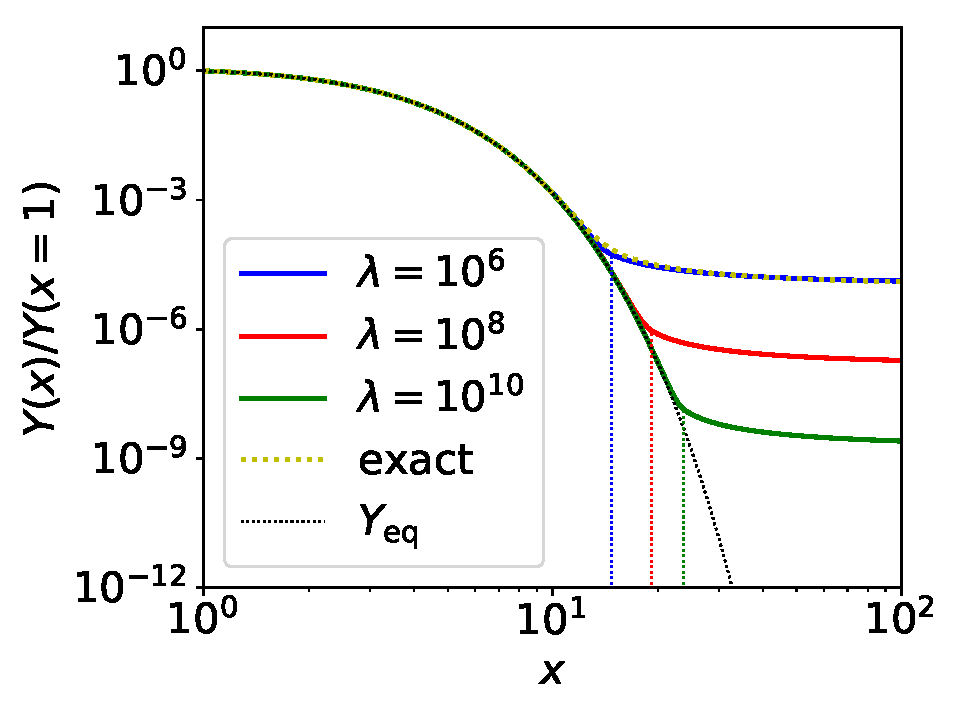
\includegraphics[width=0.5\hsize]{DMrelic.pdf}
 \caption{Plot of $Y(x) / Y(x=1)$ with $Y(x)$ being a solution of the
 evolution equation Eq.~\eqref{eq_boltzmann_Yx}.  The yellow dotted
 line is a solution for $\lambda \equiv \left. \Gamma / H
 \right|_{x=1} = 10^6$, while the black dotted line denotes
 $Y_{\mathrm{eq}} (x) / Y_{\mathrm{eq}} (x=1)$.  The solid lines are
 the approximation to the solutions described in the text.  The blue,
 red, and green colors correspond to $\lambda = 10^8$, $10^{10}$, and
 $10^{12}$, respectively.  The vertical dotted lines denote the
 freezeout temperature $x_f$.}  \label{fig_DM_relic}
\end{figure}

Here we assume that the freezeout occurs when the relativistic radiation
dominates the total energy of the universe, which will be verified to be
correct later.  In this case, we can derive $a \propto T^{-1}$ from the
entropy conservation with $s \propto T^3$.  For the numerical
calculation, we define a dimensionless parameter $x \equiv m_\chi / T$.
% Since the time dependence of $x$ is the same as $a$, $\dot{x} = x H$
% with $H$ being the Hubble parameter.  In addition, $H \propto \rho^{1/2}
% \propto x^{-2}$ and $s \propto x^{-3}$ allows us to extract the $x$
% dependence as $H(x) = H(x=1) x^{-2}$ and $s(x) = s(x=1) x^{-3}$,
% respectively.
Then we can rewrite Eq.~\eqref{eq_boltzmann_Yt} as
\begin{align}
 \frac{x}{Y_{\mathrm{eq}}} \frac{d Y}{d x} =
 -\frac{\Gamma}{H} \left( \frac{Y^2}{Y_{\mathrm{eq}}^2} - 1 \right),\label{eq_boltzmann_Yx}
\end{align}
where $\Gamma$ denotes the DM interaction rate defined as
\begin{align}
 \Gamma &\equiv n_{\mathrm{eq}} \Braket{\sigma v}.\label{eq_lambda}
\end{align}
Finally, $\Braket{\sigma v}$ is known to be expanded
as~\cite{Gondolo:1990dk}
\begin{align}
 \Braket{\sigma v} = \Braket{\sigma v}_s +
 \Braket{\sigma v}_p x^{-1} + \cdots,
\end{align}
collesponding to the $s$-wave, $p$-wave, and so on, contributions to
the cross section.  When $x \gg 1$, the term with the highest power of
$x$ dominates the cross section.  When the $x^{-p}$ term dominates ($p
\geq 0$), temperature dependence of the interaction rate is $\Gamma
\propto x^{-3/2-p} e^{-x}$, while the Hubble parameter only reduces as
$H \propto \rho^{1/2} \propto x^{-2}$.  As a result, at some point
$\Gamma$ becomes smaller than $H$ and $Y$ freezes out as
Eq.~\eqref{eq_boltzmann_Yx} indicates.  Hereafter, we focus on the
case of the $s$-wave domination with $\Braket{\sigma v}_s \neq 0$ for
simplicity.  \rem{What is the difference for $p$-wave and so on?}  In
Fig.~\ref{fig_DM_relic}, we show the solution of
Eq.~\eqref{eq_boltzmann_Yx} for $\lambda \equiv \left. \Gamma / H
\right|_{x=1} = 10^6$ by the yellow dotted line.  In the calculation,
we use the boundary condition $Y(x=1) = Y_{\mathrm{eq}} (x=1)$ and
plot the normalized value $Y(x) / Y(x=1)$.  We also plot the function
$Y_{\mathrm{eq}} (x) / Y_{\mathrm{eq}} (x=1)$ by the black dotted line.

Unfortunately, it is computationally hard to solve
Eq.~\eqref{eq_boltzmann_Yx} for larger values of $\lambda$ because of
the almost complete cancellation between two terms of the right handed
side for small $x\sim \mathcal{O}(1)$ and its amplification caused by
large $\lambda$.  We adopt instead to use an approximation that is the
same with the one adopted in the public code
\texttt{MicrOMEGAs}~\cite{Belanger:2001fz, Belanger:2018mqt}.  For the
small $x$ region, temperature is still high enough to maintain the
equilibrium $Y \simeq Y_{\mathrm{eq}}$, which means that $d \Delta Y / d
x \ll d Y_{\mathrm{eq}} / d x$ with $\Delta Y \equiv Y -
Y_{\mathrm{eq}}$.  From this approximation we obtain a formula
\begin{align}
 \Delta Y \simeq -\frac{x}{2 \lambda} \frac{d Y_{\mathrm{eq}}}{d x}.\label{eq_relic_app_1}
\end{align}
Then we define the time $x_f$, or equivalently the so-called freezeout
temperature $T_f$, when the approximation becomes invalid through the
equation
\begin{align}
 \Delta Y (x_f) = 2.5 Y_{\mathrm{eq}} (x_f).
\end{align}
After the freezeout $x > x_f$, the annihilation of the DM pairs
rapidly slows down and the DM abundance far exceeds its equilibrium
value: $Y \gg Y_{\mathrm{eq}}$.  Then we can neglect the second term
of the right hand of Eq.~\eqref{eq_boltzmann_Yx} and obtain the
analytical solution
\begin{align}
 Y(x) \simeq - \frac{x}{c_1 x + \lambda / Y_{\mathrm{eq}} (x=1)},\label{eq_relic_app_2}
\end{align}
where $c_1$ is a integration constant.  In Fig.~\ref{fig_DM_relic}, we
show results obtained with these two approximations
Eqs.~\eqref{eq_relic_app_1} and \eqref{eq_relic_app_2} for $\lambda =
10^6$ (blue), $10^8$ (red), and $10^{10}$ (green).  In particular,
the blue and the yellow lines almost completely overlaps with each
other, which proves the validity of the approximations.  The vertical
dotted lines in the figure show the freezeout temperature.  It can be
seen from the figure that $x = x_f$ does correspond to the time when $Y$
starts to deviate from $Y_{\mathrm{eq}}$.  Note also that as $\lambda
\propto \Braket{\sigma v}$ becomes larger, the freezeout time becomes
later and the late time relic abundance becomes smaller.

When the DM properties (\textit{i.e.}, the mass $m_\chi$ and the
annihilation cross section $\Braket{\sigma v}$) are given,
corresponding relic abundance can be calculated using above procedure.
In particular, $m_\chi$ determines the normalization of the figure,
namely $Y_{\mathrm{eq}} (x=1) = Y_{\mathrm{eq}} (T=m_\chi)$, and
$\Braket{\sigma v}$ determines the freezeout temperature through the
combination of Eq.~\eqref{eq_lambda}.  Assuming the absence of
non-thermal effect, only some good combination of these two values
should explain the current relic abundance of the DM.  From the
numerical calculation, we obtain an order estimation formula
\begin{align}
 \Omega_\chi h^2 \sim \frac{3 \times 10^{-27}\,\mathrm{cm^3}/\mathrm{s}}
 {\Braket{\sigma v}_0} \sim
 0.1 \left( \frac{0.01}{\alpha} \right)^2
 \left( \frac{m_\chi}{300\,\mathrm{GeV}} \right)^2,\label{eq_relic_abundance}
\end{align}
where the rough estimation $\Braket{\sigma v} \sim \alpha^2/m_\chi^2$
is used in the last equation with $\alpha$ being the fine structure
constant for the DM-SM coupling.  What is fascinating in
Eq.~\eqref{eq_relic_abundance} is that an object can be a DM candidate
if it has mass comparable to the electroweak scale and coupling
constant comparable to the electroweak coupling constant.  This is the
so-called \textit{WIMP miracle}, which suppport the hypothesis of the
WIMP as a cadidate of the DM.  Such $\mathrm{TeV}$-scale WIMPs are
theoretically well-motivated in connection with problems of the SM
such as the naturalness problem.  Several examples are briefly
reviewed in the next section.

%%%%%%%%%%%%%%%%%%%%%%%%%%%%%%%%%%%%%%%%%%%%%%%%%%%%%%%%%%%%%%%%%%%%%%%%%%%%%%%
\subsection{WIMP DM search : indirect detection}
%%%%%%%%%%%%%%%%%%%%%%%%%%%%%%%%%%%%%%%%%%%%%%%%%%%%%%%%%%%%%%%%%%%%%%%%%%%%%%%



%%%%%%%%%%%%%%%%%%%%%%%%%%%%%%%%%%%%%%%%%%%%%%%%%%%%%%%%%%%%%%%%%%%%%%%%%%%%%%%
\subsection{WIMP DM search : direct detection}
%%%%%%%%%%%%%%%%%%%%%%%%%%%%%%%%%%%%%%%%%%%%%%%%%%%%%%%%%%%%%%%%%%%%%%%%%%%%%%%



% \bibliographystyle{elsarticle-num}
% \bibliography{../phd}

\end{document}
